% Chapter Template

\chapter{Ensayos y Resultados} % Main chapter title

\label{Chapter4} % Change X to a consecutive number; for referencing this chapter elsewhere, use \ref{ChapterX}

Este capítulo expone las características del dispositivo desarrollado en contraste con los requerimientos de diseño y los casos de uso.
%----------------------------------------------------------------------------------------
%	SECTION 1
%----------------------------------------------------------------------------------------

\section{Análisis de casos de uso y cumplimiento de los requerimientos}
\label{sec:pruebasHW}

\textbf{Caso de uso CU001: Autonomía}

El primer caso de uso analizado está relacionado a la autonomía del equipo. Se midió el consumo del equipo en diferentes situaciones en la que no está conectado por USB. Los resultados se muestran en la Tabla \ref{tab:autonomia}.

\begin{table}[h]
\caption{Autonomía del Equipo}
\label{tab:autonomia}
\begin{tabular}{@{}llll@{}}
\toprule
\textbf{Fase}                       & \textbf{\begin{tabular}[c]{@{}l@{}}Consumo\\ promedio\end{tabular}} & \textbf{\begin{tabular}[c]{@{}l@{}}Duración \\ estimada\end{tabular}} & \textbf{Descripción}                                                                                                \\ \midrule
En espera de conexión BT                  & I$_0$ = 78mA                                                         & t$_0$ = 30 min                                                         & \begin{tabular}[c]{@{}l@{}}Instalo el equipo y \\ conecto sensores\end{tabular}                                     \\
Configuración previa a experiencia  & I$_1$ = 65mA                                                         & t$_1$ = 30 min                                                          & \begin{tabular}[c]{@{}l@{}}Envío señal de prueba, \\ configuro parámetros\end{tabular}                              \\
Equipo conectado BT inactivo        & I$_2$ = 62 mA                                                        & t$_2$ = 10 min                                                          & \begin{tabular}[c]{@{}l@{}}Modificación de la \\ instalación del equipo \\ (sujeción, conectores, etc)\end{tabular} \\
Equipo adquiriendo sin enviar señal & I$_3$ = 45 mA                                                        & t$_3$ = 24 hs                                                           & Experiencia                                                                                                         \\
Acceso a ver señal                  & I$_4$ = 75 mA                                                       & t$_4$ = 20 min                                                           & \begin{tabular}[c]{@{}l@{}}Accedo eventualmente a \\ ver la señal que se está\\ adquiriendo\end{tabular}            \\ \bottomrule
\end{tabular}
\end{table}

Se calculó el consumo medio teórico realizando el promedio ponderado de los consumos en las situaciones presentadas en la Tabla \ref{tab:autonomia}. El resultado se presenta en la ecuación \ref{eqn:consumoMedio}.

\begin{equation} \label{eqn:consumoMedio}
consumoMedio = I_{0}*t_{0}+I_{1}*t_{1}+I_{2}*t_{2}+I_{3}*t_{3}+I_{4}*t_{4} = 1186.3 mAh
\end{equation}



Asimismo, la corriente media se puede calcular dividiendo por el tiempo total, como se muestra en la ecuación\ref{eqn:corrienteMedia}. A partir de este dato es posible estimar la eficiencia del regulador para esa tensión.

\begin{equation} \label{eqn:corrienteMedia}
I_{med} = \frac{I_{0}*t_{0}+I_{1}*t_{1}+I_{2}*t_{2}+I_{3}*t_{3}+I_{4}*t_{4}}{t_{0}+t_{1}+t_{2}+t_{3}+t_{4}}= 46.54mA
\end{equation}

De acuerdo a la hoja de datos del regulador TPS63001 \citep{texas2006}, esta corriente media da una eficiencia de alrededor de 90\%, aunque este valor también depende de la tensión de la batería.
Se colocó en el equipo una batería en serie modelo TR18650 de 3.7V con una autonomía de 2400mAh, como muestra la figura \ref{fig:bateria}. El cálculo se realizó suponiendo una descarga lineal de la misma, desde su tensión inicial hasta la mínima tensión admisible para el regulador, que es de 1.8V\citep{texas2006} (este valor fue comprobado experimentalmente). El porcentaje de descarga de la batería antes de que el regulador deje de funcionar se calcula en la Ecuación \ref{eqn:porcentajeDescarga}.

\begin{equation} \label{eqn:porcentajeDescarga}
porcentajeDescarga = \frac{V_{ini} - V_{fin}}{V_{ini}} * 100\% = \frac{3.7V- 1.8V}{3.7V} * 100\% = 51.35\%
\end{equation}

\begin{figure}[!htbp]
	\centering	
	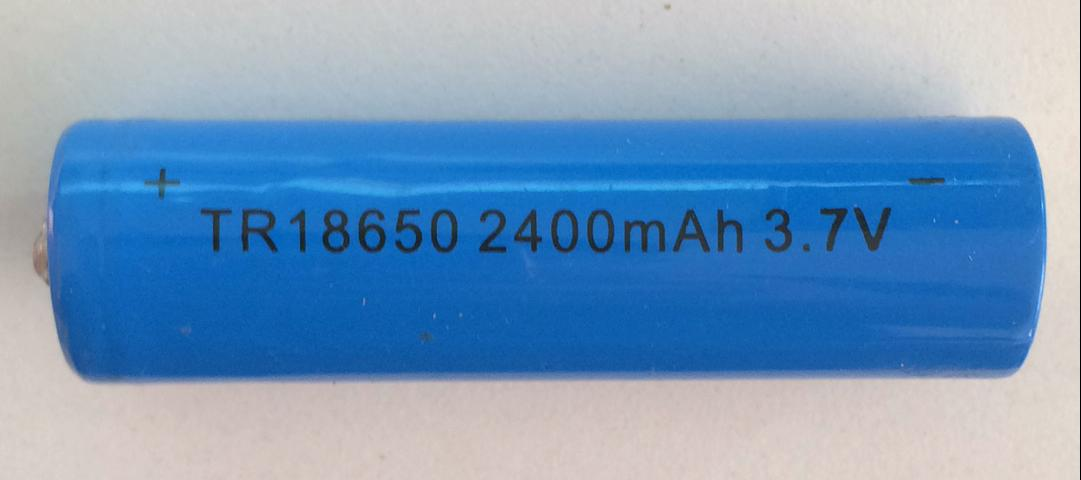
\includegraphics[width=0.5\textwidth]{./Figures/bateria.jpeg}			
	\caption{Batería TR18650 utilizada en el equipo}
	\label{fig:bateria}
\end{figure}

Teniendo en cuenta la eficiencia del 90\% y el porcentaje de descarga máxima de 51.35\%, la autonomía aprovechable de la batería será aproximadamente de 1109mAh, según lo calculado en la Ecuación \ref{eqn:autonomiaReal}.


\begin{equation} \label{eqn:autonomiaReal}
\begin{split}
autonomiaReal = autonomiaReal*eficiencia*porcentajeDescarga = \\ 2400mAh * 90\% * 51.35\% = 1109 mAh
\end{split}
\end{equation}

Este valor es cercano al consumo teórico calculado en \ref{eqn:consumoMedio}.
Se realizaron varias experiencias para verificar la autonomía del equipo y se obtuvieron en todas resultados similares. La duración de la batería fue de aproximadamente 22 horas. Puede verse la curva de descarga de una de las experiencias en la figura \ref{fig:descargaBateria}. En esta figura se decimaron las muestras obtenidas y se visualiza una medición cada media hora. El divisor resistivo de entrada del ADC conectado a la batería es de 330kOhm y 820kOhm, lo que da una relación de 0.287. Este valor se usó para convertir las muestras entregadas por el ADC a Volts.

\begin{figure} [!htpb]
    \centering
    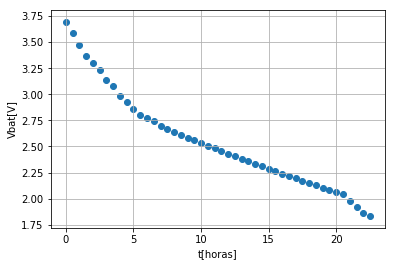
\includegraphics[width=\textwidth]{./Figures/descargaBateria.png}
    \caption{Descarga de la bateria durante experiencia}
    \label{fig:descargaBateria}
\end{figure}

Los requerimientos asociados a este caso de uso no son cubiertos completamente. Sin embargo, se puede solucionar colocando una batería de mayor autonomía como puede ser la indicada en \citep{rs2019}, que no fue adquirida por una cuestión de presupuesto.


\textbf{Caso de uso CU002: Configuración}

Para comprobar este caso de uso se inició con el equipo reiniciado por hardware. Se utilizó una tablet con Android y la aplicación Bluterm instalada. A través de la aplicación se enviaron los comandos para ingresar al modo configuración, y luego se modificaron cada uno de los parámetros, comprobando la escritura en las variables asociadas en RAM a través del debugger. Luego se realizaron diferentes mediciones para distintas configuraciones. Estas mediciones fueron realizadas con señales provistas por un generador de señales UTG4082A excitando la entrada del amplificador operacional. En la figura \ref{fig:confPGA} puede visualizarse la misma señal generada adquirida con dos ganancias de PGA diferentes (1 y 2). El setup para la experiencia puede visualizarse en la figura \ref{fig:confPGAexp}.

\begin{figure} [!htpb]
    \centering
    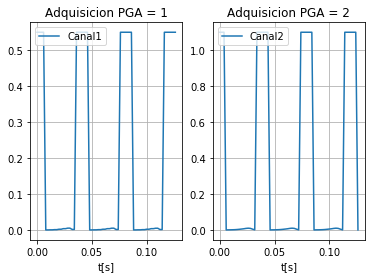
\includegraphics[width=\textwidth]{./Figures/confPGA.png}
    \caption{Señales adquiridas con PGA = 1 y PGA = 2}
    \label{fig:confPGA}
\end{figure}

\begin{figure} [!htpb]
    \centering
    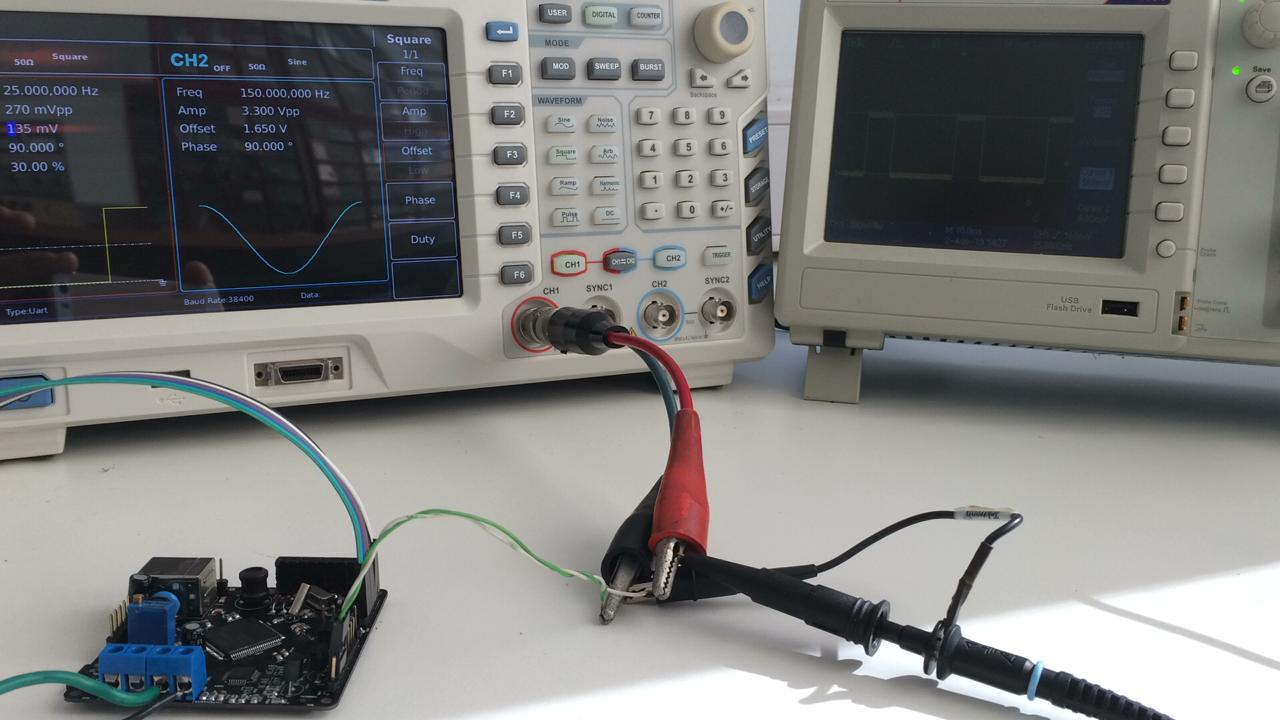
\includegraphics[width=\textwidth]{Figures/confPGAexp.jpeg}
    \caption{Señales adquiridas con PGA = 1 y PGA = 2}
    \label{fig:confPGAexp}
\end{figure}

Se realizó igualmente la configuración de habilitación de un solo canal (canal 1 y canal 2 por separado), la configuración de fecha y hora, y el muestreo a frecuencias de 500SPS, 250SPS y 125SPS.

También se realizó la rutina de calibración con uno de los sensores Königsberg, pero sin contar con un patrón de calibración de presión. Se comprobó unicamente la adquisición de valores diferentes de presión aplicando presión con el dedo y visualizando una medición mayor con su correspondiente incremento en el valor adquirido. El setup puede visualizarse en la figura \ref{fig:calibracion}. Resta comprobar la calibración con un patrón certificado de presión que sea adaptable a los sensores a utilizar. 

\begin{figure} [!htpb]
    \centering
    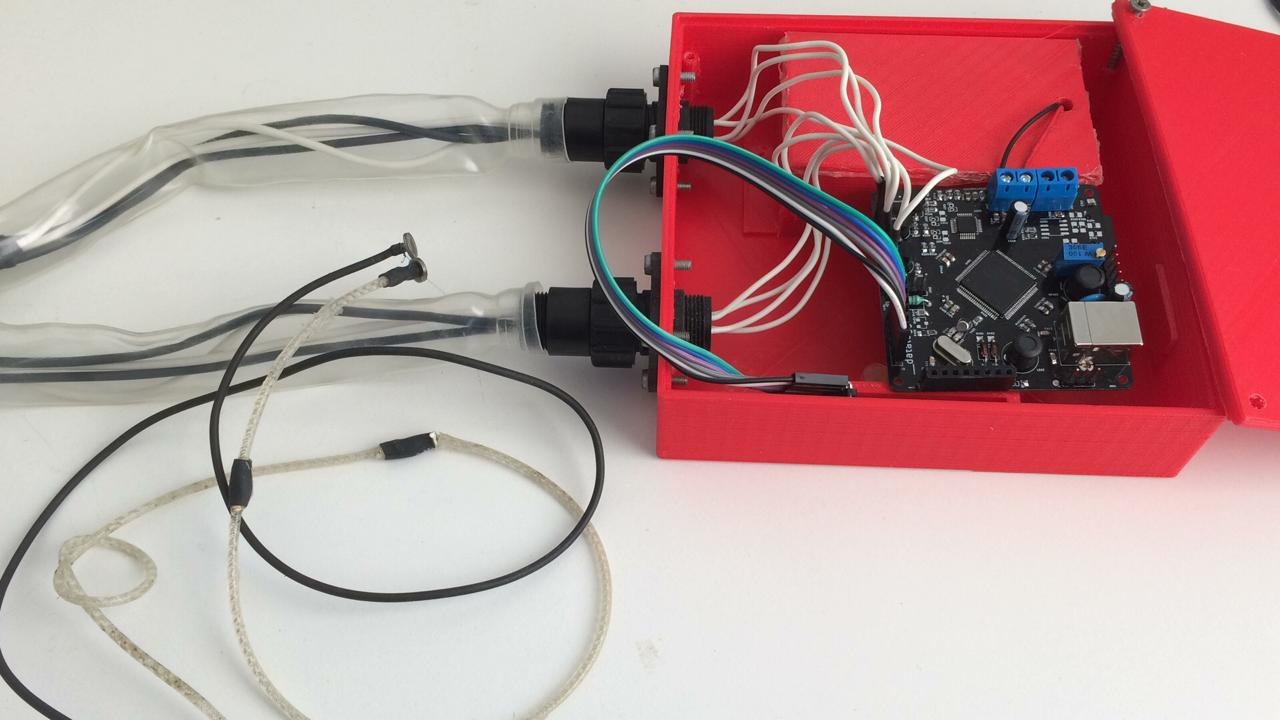
\includegraphics[width=\textwidth]{./Figures/calibracion.jpeg}
    \caption{Setup para calibración con sensores Königsberg}
    \label{fig:calibracion}
\end{figure}

\textbf{Caso de uso CU003: Experiencia}

Para este caso de uso se cargó la batería al 100\% y se operó el dispositivo desde una terminal con Android, utilizando la aplicación Bluterm. Por tratarse de una prueba de funcionamiento, se utilizó el mismo setup que en el caso de la calibración, es decir, con los sensores a presión atmosférica. Se ingresó en el modo de ''adquirir+enviar'', con la configuración por default, es decir, con los dos canales habilitados, el PGA en ganancia unitaria, y una frecuencia de muestreo de 500SPS. 

Se comprobó el correcto envío de muestras truncadas a 16 bits y decimadas a 100Hz para no sobrecargar el módulo Bluetooth. Luego se pasó al modo ''adquirir+enviar+almacenar'' y finalmente al modo ''adquirir+almacenar''. Después de esperar cinco minutos, se interrumpió la experiencia para comprobar el correcto almacenamiento en la memoria micro SD. 
Se volvió a comenzar la experiencia de la misma manera pero esta vez no se interrumpió el almacenamiento y se continuó por 20 horas, finalmente se dio por terminada la experiencia. 

Esta secuencia se repitió pero intercalando ingresos a través de la aplicación Bluterm para consultar el envío de la señal online, de manera de comprobar que la visualización de la señal no altere el almacenamiento en la SD.
Se repitió el mismo procedimiento por cuarta vez, pero ahora utilizando el generador de señales para comprobar la adquisición de una señal conocida. 

La estrategia elegida para almacenar las señales fue generar archivos de hasta 50Mb para evitar problemas de copia o corrupción. Para obtener mejor rendimiento de velocidad al escribir y menor volumen de datos, toda la información se guardó en formato binario. En cada uno de los archivos se guardo información que contiene un número de identificación de la experiencia autonumerado, un índice que comienza en cero y que indica el número de archivo generado abierto durante la experiencia, la fecha en que se guardó el archivo, hora de inicio del archivo, valor de ganancia del PGA, cantidad de canales habilitados, y valor de la frecuencia de muestreo. En cada una de las muestras se guardaron tres bytes por cada muestra por cada canal, ya que el ADC es de 24 bits y no tiene sentido guardar los cuatro bytes de la variable donde se almacenan los valores. Además para cada valor se guarda un byte correspondientes a la batería, truncando la muestra de 12 bits del ADC interno. La información de hora y fecha solamente se guarda en el encabezado, y no en cada muestra.

Para poder visualizar estos archivos se creó un script de python que reune esta información y la escribe en un formato legible, además compagina todos los archivos generados por la experiencia, graficando las señales. Este script se realizó con fines de desarrollo, ya que la aplicación para visualización e interfaz con el equipo no alcanza los objetivos del presente trabajo. 

Resta por realizar las pruebas de aceptación en un caso real, con un animal instrumentado. Esta experiencia no pudo ser realizada dado los costos e impedimentos operativos, pero se planifica realizar en el corto plazo.

\textbf{Caso de uso CU004: Descarga de datos y carga de batería}

En todos las experiencias realizadas para el CU003 se descargaron los archivos via USB. Para el tamaño de archivos que se maneja no hubo ningún inconveniente y el equipo respondió correctamente.

La carga de batería se realiza una corriente constante de 100mA, por lo que una carga completa con la batería totalmente descargada toma 24 horas. En todos los casos, luego de cargar la batería, se comprobó que la tensión final de carga sea 3.7V utilizando un tester UNI-T PRO UT195DS. 

\section{Ensayos adicionales}

También se realizaron ensayos para cubrir los requerimientos no funcionales, como los relacionados a las dimensiones físicas del equipo R2.1, R2.2 y R2.3. 

\begin{itemize}

\item R2.1: se hizo el pesaje del equipo en una balanza comercial. El peso con los sensores y el gabinete es de aproximadamente 366 gramos. 

\item R2.2: el gabinete del equipo mide 13.5cm x 12.8cm, más 1.5cm en la arista que contiene los conectores para los sensores. Este gabinete fue reutilizado de una versión anterior y cuenta con un gran espacio disponible en su interior, por lo que, si bien este requerimiento no fue cubierto en su totalidad, puede cumplirse realizando un nuevo gabinete, ya que el volumen que ocupa el circuito impreso y las baterías es mucho menor.

\item R2.3: durante todas las fases de los ensayos realizados se prestó especial atención a la temperatura de los compontentes. En ningún caso, ninguno de los componentes del circuito llegó tener una temperatura significativamente superior a la ambiental. Esto es consistente con el bajo consumo de corriente. El módulo Bluetooth es la única parte del sistema que llega a tener una temperatura apenas perceptiblemente mayor. 


\end{itemize}

\section{Resumen de los resultados} \label{resumenResultados}

A continuación en la Tabla \ref{tab:tablaConformidad} se sintetiza toda la información anterior: se muestra una lista de los requerimientos iniciales y su grado de conformidad.

\pagebreak

\footnotesize
\begin{longtable}[c]{lll}
\caption{Tabla de conformidad de requerimientos}\\ 
\hline
\textbf{REQ/CU} & \textbf{Conformidad} & \textbf{Observaciones}                                                                                                                                                                                                                                    \\ \hline
%
\endhead
%
R1.1            & Parcial              & \begin{tabular}[c]{@{}l@{}}Se debe colocar una batería \\ de mayor autonomía para superar\\ las 24hs de adquisición.\end{tabular}                                                                                                                         \\ \hline
R1.2            & Completa             & -                                                                                                                                                                                                                                                         \\ \hline
R2.1            & Completa             & -                                                                                                                                                                                                                                                         \\ \hline
R2.2            & Parcial              & \begin{tabular}[c]{@{}l@{}}Se debe cambiar el gabinete por\\ un nuevo diseño ya que el espacio\\ del circuito impreso y las baterías\\ es mucho menor al actual.\end{tabular}                                                                             \\ \hline
R2.3            & Completa             & -                                                                                                                                                                                                                                                         \\ \hline
R3.1            & Completa             & -                                                                                                                                                                                                                                                         \\ \hline
R3.2            & Completa             & -                                                                                                                                                                                                                                                         \\ \hline
R3.3            & Completa             & -                                                                                                                                                                                                                                                         \\ \hline
R4.1            & Parcial              & \begin{tabular}[c]{@{}l@{}}La resolución del ADS1292 y el nivel de\\ ruido del equipo permiten inferir que\\ este requisito es factible de cumplir, sin embargo,\\ es necesario realizar una calibración de los\\ sensores para comprobarlo.\end{tabular} \\ \hline
R4.2            & Completa             & \begin{tabular}[c]{@{}l@{}}Se realizaron pruebas con memorias de 2GB que \\ superan ampliamente el tamaño del paquete de \\ archivos generados por una experiencia de 24hs\\ con dos canales en 24 bits.\end{tabular}                                     \\ \hline
R4.3            & No Completa          & Este requerimiento resultó irrelevante en la práctica                                                                                                                                                                                                     \\ \hline
R5.1            & Completa             & -                                                                                                                                                                                                                                                         \\ \hline
R5.2            & Completa             & \begin{tabular}[c]{@{}l@{}}El ADS1292 cuenta con conversores A/D, que \\ toman las muestras con el mismo timer de entrada\end{tabular}                                                                                                                    \\ \hline
R6.1            & Completa             & -                                                                                                                                                                                                                                                         \\ \hline
R6.2            & Completa             & -                                                                                                                                                                                                                                                         \\ \hline
R6.3            & Completa             & -                                                                                                                                                                                                                                                         \\ \hline
R6.4            & Completa             & -                                                                                                                                                                                                                                                         \\ \hline
R6.5            & Completa             & -                                                                                                                                                                                                                                                         \\ \hline
R6.6            & Completa             & -                                                                                                                                                                                                                                                         \\ \hline
R6.7            & Completa             & -                                                                                                                                                                                                                                                         \\ \hline
R6.8             & Completa             & -                                                                                                                                                                                                                                                         \\ \hline
R6.9            & Completa             & -                                                                                                                                                                                                                                                         \\ \hline
R6.10           & Completa             & -                                                                                                                                                                                                                                                         \\ \hline
R6.11           & Completa             & -                                                                                                                                                                                                                                                         \\ \hline
R6.12           & Completa             & \begin{tabular}[c]{@{}l@{}}Se optó por registrar fecha y hora en el encabezado\\ de cada archivo en lugar de cada registro.\end{tabular}                                                                                                                  \\ \hline
R6.13           & Completa             & \begin{tabular}[c]{@{}l@{}}Se optó por generar varios archivos de 50Mb por cada \\ registro\end{tabular}                                                                                                                                                  \\ \hline
R6.14           & Completa             & -                                                                                                                                                                                                                                                         \\ \hline
R6.15           & Completa             & \begin{tabular}[c]{@{}l@{}}El led es SMD y se debería colocar en su lugar un \\ led THT visible desde fuera del gabinete.\end{tabular}                                                                                                                    \\ \hline
R7.1            & Completa             & -                                                                                                                                                                                                                                                         \\ \hline
R7.2            & Completa             & -                                                                                                                                                                                                                                                         \\ \hline
R7.3            & Completa             & -                                                                                                                                                                                                                                                         \\ \hline
R7.4            & Completa             & -                                                                                                                                                                                                                                                         \\ \hline
R7.5            & Completa             & -                                                                                                                                                                                                                                                         \\ \hline
R7.6            & Parcial              & \begin{tabular}[c]{@{}l@{}}Resta por realizar la calibración contra un patrón\\ de presión
\end{tabular}                                                                                                                                                     \\ \hline
\label{tab:tablaConformidad}
\end{longtable}
\normalsize

